\documentclass[aspectratio=169,11pt]{beamer} % 16:9 aspect ratio, slightly larger font
\usepackage[T1]{fontenc}          % keeps hyphen-ation right in pdfLaTeX
\usetheme{default}  % Metropolis beamer theme
\usepackage{tikz}
\usetikzlibrary{calc, decorations.pathreplacing}
\usepackage{amsmath,amssymb}
\DeclareMathOperator*{\E}{\mathbb{E}}
\newcommand{\indep}{\perp\!\!\!\perp} % independence symbol
\beamerdefaultoverlayspecification{<+->}
\setbeamerfont{frame title}{size=\large}
\setbeamersize{text margin left=5pt,text margin right=5pt}

\setbeamerfont{itemize/enumerate body}{size=\small}
\setbeamerfont{itemize/enumerate subbody}{size=\footnotesize}


\title{Probability Lecture}
\subtitle{Conditional Probability, Independence, and Beyond}
\author{Instructor Name}
\date{}

\begin{document}

\maketitle

\section{Conditional Probability}

\begin{frame}{Motivating Example 1/3}
Consider a fair six-sided die.\\[1ex]
\begin{itemize}
    \item Given that we rolled an \emph{even} number, what is the probability that we rolled a 2?
    \item What is the probability that we rolled a 3?
\end{itemize}
\end{frame}
\begin{frame}{Example 1 — Solution}
If we know the outcome is even ($\{2,4,6\}$), the conditional space contains three equally likely outcomes.  
Therefore  
\[
P(\text{rolled 2}\mid\text{even})=\frac{1}{3},\qquad
P(\text{rolled 3}\mid\text{even})=0.
\]
\end{frame}



\begin{frame}{Motivating Example 2/3}
Suppose the same fair die rolled a number \emph{greater than 3}. What is the probability that:
\begin{itemize}
    \item the outcome was an \emph{even} number?
    \item it was a 4? A 3?
\end{itemize}
\end{frame}
\begin{frame}{Example 2 — Solution}
Given the outcome is $>3$ ($\{4,5,6\}$), we again have three equally likely cases.  
Thus
\[
P(\text{even}\mid>3)=\frac{|\{4,6\}|}{|\{4,5,6\}|}=\frac23,\qquad
P(4\mid>3)=\frac13,\quad P(3\mid>3)=0.
\]
\end{frame}



\begin{frame}{Motivating Example 3/3}
Now roll two fair dice. Knowing that their sum is $\le 5$, determine the probability that:
\begin{itemize}
    \item one of the dice shows a 5. What about a 4?
    \item the \emph{first} die shows a 2?
    \item at least one die shows a 2?
\end{itemize}
\end{frame}
\begin{frame}{Example 3 — Solution}
Let $B=\{\text{sum}\le5\}$.  Enumerating all $10$ outcomes in $B$:
\[
\begin{array}{c|cccccccccc}
(1,1)&(1,2)&(1,3)&(2,1)&(2,2)&(2,3)&(3,1)&(3,2)&(4,1)&(2,2)
\end{array}
\]
Among these $10$ equally likely outcomes:
\begin{itemize}
  \item \emph{No} pair shows a 5, so $P(\text{a 5}\mid B)=0$ while $P(\text{a 4}\mid B)=2/10=1/5$.
  \item Three outcomes have first die $=2$ $\Rightarrow P(\text{first die 2}\mid B)=3/10$.
  \item Five outcomes contain at least one 2 $\Rightarrow P(\text{some 2}\mid B)=1/2$.
\end{itemize}
\end{frame}


% Solutions moved to individual frames


\begin{frame}{Definition of Conditional Probability}
\large
Given two events $A$ and $B$ with $P(B) > 0$, the \textbf{conditional probability} of $A$ \emph{given} $B$ is defined as:
\[ P(A \mid B) = \frac{P(A \cap B)}{P(B)}.\]

In words: $P(A \mid B)$ is the probability that $A$ occurs \emph{under the assumption that $B$ has occurred}. \\[1ex]

Equivalently, once we know $B$ happened, we ``restrict'' our sample space to $B$ and renormalize probabilities so the total within $B$ is 1.
\end{frame}

\begin{frame}{Checking the Examples}
Using $P(A \mid B) = P(A \cap B)/P(B)$, we can verify our answers:
\begin{itemize}
  \item Example 1: $A=\{\text{roll 2}\}, B=\{\text{even}\} = \{2,4,6\}.$ 
  \[P(2 \mid \text{even}) = \frac{P(\{2\} \cap \{2,4,6\})}{P(\{2,4,6\})} = \frac{P(\{2\})}{P(\{2,4,6\})} = \frac{1/6}{3/6} = \frac{1}{3}.\] 
  Similarly, $P(3 \mid \text{even}) = \frac{0}{3/6} = 0.$
  \item Example 2: $B=\{4,5,6\}, A=\{\text{even}\}=\{2,4,6\}.$ 
  \[P(\text{even} \mid >3) = \frac{P(\{4,6\})}{P(\{4,5,6\})} = \frac{2/6}{3/6} = \frac{2}{3}.\] 
  And $P(4 \mid >3) = \frac{1/6}{1/2} = 1/3,$ $P(3 \mid >3)=0.$
  \item Example 3: $B=\{\text{sum}\le5\}$ (10 outcomes). $A_1=\{\text{a die is 4}\}$, $P(A_1 \cap B) = 2/36, P(B)=10/36 \implies P(A_1 \mid B) = 2/10 = 0.2.$ 
  Similarly $P(\text{first die is 2} \mid B) = 3/10,$ and $P(\text{at least one 2} \mid B) = 5/10.$
\end{itemize}
\end{frame}

\begin{frame}{Sanity Checks}
Some quick sanity checks (for $P(B)>0$):
\begin{itemize}
    \item $P(B \mid B) = \frac{P(B \cap B)}{P(B)} = 1.$ (If we condition on $B$, the probability $B$ occurred is 1.)
    \item $P(\emptyset \mid B) = \frac{P(\emptyset)}{P(B)} = 0.$ (Given $B$, an impossible event still has probability 0.)
    \item $P(\Omega \mid B) = \frac{P(\Omega \cap B)}{P(B)} = \frac{P(B)}{P(B)} = 1.$ (The whole space event always occurs given $B$.)
    \item If $A^c$ is the complement of $A$, then $P(A^c \mid B) = 1 - P(A \mid B)$.
\end{itemize}
\end{frame}

\begin{frame}[fragile]{Properties of Conditional Probability}
\textbf{Basic Properties:} For any events $A, B, C$ with $P(C)>0$:
\begin{itemize}
    \item $0 \le P(A \mid C) \le 1.$
    \item If $A \subseteq B$, then $P(A \mid C) \le P(B \mid C).$
    \item $P(A \mid C) + P(A^c \mid C) = 1.$
    \item $P(A \setminus B \mid C) = P(A \mid C) - P(A \cap B \mid C).$
\end{itemize}

\textbf{Additivity:} If $A_1, A_2, \dots$ are disjoint events, then:
\[ P\Big(\bigcup_{j} A_j \,\Big|\, C\Big) = \sum_{j} P(A_j \mid C).\] 
(Think of $P(\cdot \mid C)$ as a probability measure on $C$ itself. The additivity axiom still holds under the conditioning.)
\end{frame}

\begin{frame}{Countable Additivity Proof}
\small
Fix $C$ with $P(C)>0$. Define 
\[ Q(E) := \frac{P(E \cap C)}{P(C)}, \] 
for any event $E$. \\[1ex] 
Then $Q(\cdot)$ is a probability measure on $C$. If $\{A_j\}$ are disjoint:
\begin{align*}
Q\Big(\bigcup_j A_j\Big) &= \frac{P\Big((\bigcup_j A_j)\cap C\Big)}{P(C)} 
= \frac{P\big(\bigcup_j (A_j \cap C)\big)}{P(C)} \\
&= \frac{\sum_j P(A_j \cap C)}{P(C)} 
= \sum_j \frac{P(A_j \cap C)}{P(C)} \\
&= \sum_j Q(A_j).
\end{align*}
Thus $P(\bigcup_j A_j \mid C) = \sum_j P(A_j \mid C)$. In other words, $P(\cdot \mid C)$ is countably additive.
\end{frame}

\begin{frame}[fragile]{Example: State of Origin}
\small
In a best-of-3 series, suppose each game is equally likely to be won by the Blues (B) or Maroons (M). All $2^3 = 8$ possible win sequences are equally likely (e.g. BBB, BBM, ..., MMM). \\[1ex]
Let $B1 = \{\text{Blues win game 1}\} = \{\text{BBB, BBM, BMB, BMM}\}$ (4 outcomes). \\
Let $BW = \{\text{Blues win the series}\} = \{\text{BBB, BBM, BMB, MBB}\}$ (Blues win $\ge 2$ games). \\

\begin{alertblock}{Why do we care?}
``Look, winning that \emph{first} game is so important—just ask any long‑suffering Blues fan.
Momentum, hoodoo, the vibe—you name it, pundits will invoke it.
Queensland bellows “Queenslander!” while NSW talk themselves into a lather.''
\end{alertblock}

We have:
\begin{itemize}
    \item $P(BW \cap B1) = P(\{\text{BBB, BBM, BMB}\}) = 3/8.$ 
    \item $P(B1) = 4/8 = 1/2.$ 
\end{itemize}
Thus:
\[ P(BW \mid B1) = \frac{P(BW \cap B1)}{P(B1)} = \frac{3/8}{1/2} = \frac{3/8}{4/8} = \frac{3}{4} = 75\%. \]

So, if a team wins the first game, their chance of winning the series is 75\%. (Sports commentators often cite: ``75\% of teams who win Game 1 win the series.'')
\end{frame}

\begin{frame}[fragile]{The Monty Hall Problem}
\textbf{Problem:} You're on a game show with 3 doors. Behind one door is a car (prize), behind the others are goats. You pick one door (without opening). The host, who knows where the car is, then opens a \emph{different} door, revealing a goat. You are then offered a choice: \textbf{stay} with your original door, or \textbf{switch} to the other unopened door. \newline

\textbf{Question:} To maximize your chance of winning the car, should you stay or switch?
\end{frame}

\begin{frame}[fragile]{Monty Hall: Quick Solution}
Initially, $P(\text{car behind your door}) = \frac{1}{3}$ and $P(\text{car behind one of the other two}) = \frac{2}{3}$. \newline

The host's action (always revealing a goat behind a door you didn't pick) doesn't change these initial probabilities, but it does give information. In fact:
\begin{itemize}
    \item If you \textbf{stick} with your original door, you win only if you initially picked correctly (probability $1/3$).
    \item If you \textbf{switch}, you win if your original pick was wrong (probability $2/3$).
\end{itemize}
\textbf{Conclusion:} Switching doubles your chance of winning (from 33.3\% to 66.7\%). 
\end{frame}

\begin{frame}[fragile]{Monty Hall: Detailed Analysis}
Label the doors 1, 2, 3. Suppose you initially pick Door 1. There are three equally likely scenarios:
\begin{columns}[T]
\column{0.6\textwidth}
\begin{itemize}
    \item Car is behind Door 1 (prob $1/3$): Host opens one of \#2 or \#3 at random (both goats). If you switch, you end up with a goat (lose); if you stay, you win the car.
    \item Car is behind Door 2 (prob $1/3$): Host must open Door 3 (the only remaining goat door). If you switch (to \#2), you win the car; if you stay, you lose.
    \item Car is behind Door 3 (prob $1/3$): Host opens Door 2. If you switch (to \#3), you win; if you stay, you lose.
\end{itemize}
\column{0.35\textwidth}
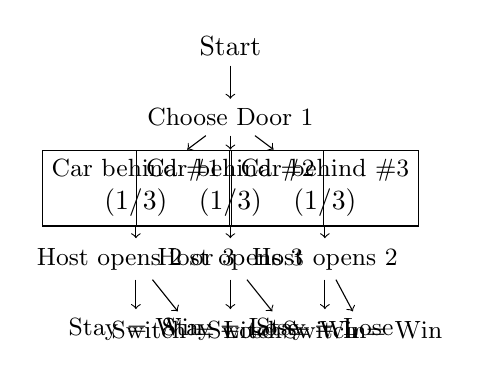
\begin{tikzpicture}[x=1.2cm,y=0.9cm]
\node (start) at (0,3) {Start};
\node (pick) at (0,2) {\small Choose Door 1};
\node[draw, rectangle, align=center] (case1) at (-1,1) {\small Car behind \#1\\(1/3)};
\node[draw, rectangle, align=center] (case2) at (0,1) {\small Car behind \#2\\(1/3)};
\node[draw, rectangle, align=center] (case3) at (1,1) {\small Car behind \#3\\(1/3)};
\node (host1) at (-1,0) {\small Host opens 2 or 3};
\node (host2) at (0,0) {\small Host opens 3};
\node (host3) at (1,0) {\small Host opens 2};
\node (stay1) at (-1,-1) {\small Stay = Win};
\node (switch1) at (-0.4,-1) {\small Switch = Lose};
\node (stay2) at (0,-1) {\small Stay = Lose};
\node (switch2) at (0.6,-1) {\small Switch = Win};
\node (stay3) at (1,-1) {\small Stay = Lose};
\node (switch3) at (1.4,-1) {\small Switch = Win};
\draw[->] (start) -- (pick);
\draw[->] (pick) -- (case1);
\draw[->] (pick) -- (case2);
\draw[->] (pick) -- (case3);
\draw[->] (case1) -- (host1);
\draw[->] (case2) -- (host2);
\draw[->] (case3) -- (host3);
\draw[->] (host1) -- (stay1);
\draw[->] (host1) -- (switch1);
\draw[->] (host2) -- (stay2);
\draw[->] (host2) -- (switch2);
\draw[->] (host3) -- (stay3);
\draw[->] (host3) -- (switch3);
\end{tikzpicture}
\end{columns}

In 2 of the 3 cases (when the car is behind \#2 or \#3), switching wins the car. So $P(\text{win|switch}) = 2/3$, whereas $P(\text{win|stay}) = 1/3$.
\end{frame}
\begin{frame}[fragile]{Monty Hall Decision Tree (big)}
\begin{center}
\scalebox{0.95}{
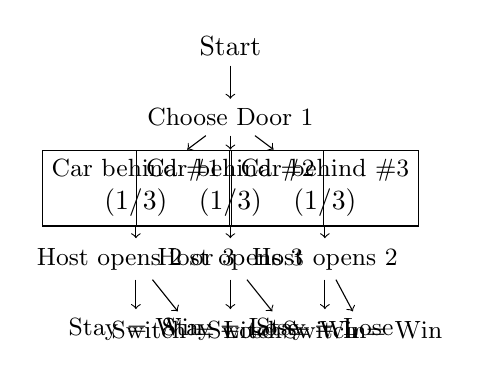
\begin{tikzpicture}[x=1.2cm,y=0.9cm]
\node (start) at (0,3) {Start};
\node (pick) at (0,2) {\small Choose Door 1};
\node[draw, rectangle, align=center] (case1) at (-1,1) {\small Car behind \#1\\(1/3)};
\node[draw, rectangle, align=center] (case2) at (0,1) {\small Car behind \#2\\(1/3)};
\node[draw, rectangle, align=center] (case3) at (1,1) {\small Car behind \#3\\(1/3)};
\node (host1) at (-1,0) {\small Host opens 2 or 3};
\node (host2) at (0,0) {\small Host opens 3};
\node (host3) at (1,0) {\small Host opens 2};
\node (stay1) at (-1,-1) {\small Stay = Win};
\node (switch1) at (-0.4,-1) {\small Switch = Lose};
\node (stay2) at (0,-1) {\small Stay = Lose};
\node (switch2) at (0.6,-1) {\small Switch = Win};
\node (stay3) at (1,-1) {\small Stay = Lose};
\node (switch3) at (1.4,-1) {\small Switch = Win};
\draw[->] (start) -- (pick);
\draw[->] (pick) -- (case1);
\draw[->] (pick) -- (case2);
\draw[->] (pick) -- (case3);
\draw[->] (case1) -- (host1);
\draw[->] (case2) -- (host2);
\draw[->] (case3) -- (host3);
\draw[->] (host1) -- (stay1);
\draw[->] (host1) -- (switch1);
\draw[->] (host2) -- (stay2);
\draw[->] (host2) -- (switch2);
\draw[->] (host3) -- (stay3);
\draw[->] (host3) -- (switch3);
\end{tikzpicture}
}
\end{center}
\end{frame}


\begin{frame}[fragile]{Monty Hall: A Variation}
What if the host doesn't pick randomly when faced with a choice? (E.g. if your initial pick is correct, host always opens the lowest-numbered goat door instead of choosing randomly.) \newline

If the host's strategy is known, you can condition on it:
\begin{itemize}
    \item If the host opens Door 3, that would only happen (under this rule) if the car was behind Door 2. So switching to Door 2 in that case wins with probability 1.
    \item If the host opens Door 2, it could mean the car is either behind Door 1 or Door 3 (each with 50\% conditional probability). In that case, switching yields a 50\% chance of winning (no better than staying).
\end{itemize}

If you always switch regardless, the overall win probability still works out to 2/3. However, an optimal strategy could be: switch only when the host opens a particular door. In general, the solution to Monty Hall-type problems depends on the host's behavior, but the classic version assumes the host opens a random goat door when able.
\end{frame}

\begin{frame}{False Positive Paradox --- Setup}
\textbf{Scenario:} A rare genetic disorder occurs in $0.1\%$ of births.  
A prenatal screening test has:
\begin{itemize}
    \item \textbf{Sensitivity:} If the fetus \emph{has} the disorder, the test is positive 100\% of the time.
    \item \textbf{Specificity:} If the fetus is \emph{healthy}, the test is negative 95\% of the time (i.e.\ a 5\% false-positive rate).
\end{itemize}
\textbf{Question:} If a randomly selected expectant mother gets a \textbf{positive} result, what is the probability that her baby actually has the disorder?
\end{frame}

\begin{frame}{False Positive Paradox --- Computation}
Let us reason with an imaginary cohort of $100\,000$ pregnancies:
\begin{itemize}
    \item \textbf{Diseased babies}: $0.001 \times 100{,}000 = 100$.
    \item \textbf{Healthy babies}: $99{,}900$.
    \item \textbf{Positive tests} break down as:
    \begin{itemize}
        \item Diseased \& positive (true positives): $100$ (sensitivity $=100\%$).
        \item Healthy \& \emph{false} positives: $5\%$ of $99{,}900 \approx 4{,}995$.
    \end{itemize}
    \item \textbf{Total positive tests}: $100 + 4{,}995 \approx 5{,}095$.
\end{itemize}
Hence
\[
P(\text{Disorder}\mid\text{Positive}) \;=\; \frac{100}{5{,}095} \;\approx\; 1.96\%.
\]
So despite a perfectly sensitive test, a positive result still means only a $\sim2\%$ chance of disease because of the tiny base rate.
\end{frame}

\begin{frame}[fragile]{Base Rate Matters}
If instead the disorder was common (say 50\% prevalence):
\begin{itemize}
    \item Diseased babies: $50{,}000$ (all test positive).
    \item Healthy babies: $50{,}000$ (false positives: $0.05 \times 50{,}000 = 2{,}500$).
    \item Total positives: $52{,}500$, of which $50{,}000$ are true.
\end{itemize}
Now $P(\text{Disorder} \mid \text{Positive}) \approx 95.2\%$. \newline

This dramatic change (2\% vs 95\%) illustrates \textbf{base rate neglect}: people often ignore prior probabilities. Always account for the base rate when interpreting diagnostic tests! \newline

\textbf{Other examples:} 
\begin{itemize}
    \item Security alarms for very rare events will trigger mostly false alarms.
    \item Drug tests in low-prevalence populations yield more false positives than true positives.
\end{itemize}
\end{frame}

\begin{frame}{The Birthday Problem}
\textbf{Question:} How many people must be in a room so that the probability of at least two sharing the same birthday exceeds 50\%?

Surprisingly, the answer is only 23 people! (Much lower than 183, which would be 50\% of 365.) \newline

\textbf{Assumptions:} 
\begin{itemize}
    \item 365 days in a year (no Feb 29).
    \item Each person's birthday is uniformly random in $\{1,\dots,365\}$, independent of others.
\end{itemize}

\textbf{Solution approach:} Compute the complement (no shared birthdays):
\begin{itemize}
    \item Let $B_n =$ event that all $n$ birthdays are distinct.
    \item $P(B_n) = \frac{365 \times 364 \times \cdots \times (365-n+1)}{365^n}.$ 
\end{itemize}
For $n=23$:
\[P(B_{23}) = \frac{365 \times 364 \times \cdots \times 343}{365^{23}} \approx 0.4927,\] 
so $P(\text{at least one match}) \approx 1 - 0.4927 = 0.5073$ (just over 50\%).
\end{frame}

\begin{frame}[fragile]{Birthday Problem: Intuition}
At $n=23$, there are $\binom{23}{2} = 253$ pairs of people. Each pair has probability $1/365$ of matching birthdays, and 253 pairs create many opportunities for a match. \newline

As $n$ grows, the chance of a match increases rapidly:
\begin{itemize}
    \item $n=10$: $\approx 12\%$ chance of a shared birthday. 
    \item $n=23$: $\approx 50.7\%$ chance.
    \item $n=30$: $\approx 70\%$ chance.
    \item $n=50$: $\approx 97\%$ chance.
\end{itemize}

This counterintuitive result is known as the \textbf{Birthday Paradox}. One implication:
\begin{itemize}
    \item In cryptography, finding two inputs with the same hash (``collision'') is easier than brute force due to the birthday paradox (birthday attack).
    \item In any large group, surprising coincidences (like shared birthdays) are more common than naive intuition suggests.
\end{itemize}
\end{frame}

\section{Independence of Events}

\begin{frame}{Definition of Independence}
Two events $A$ and $B$ are \textbf{independent} if knowing that one occurs does not change the probability of the other. Formally, $A$ and $B$ are independent if 
\[ P(A \mid B) = P(A), \] 
whenever $P(B)>0$. (Equivalently $P(B \mid A) = P(B)$.) \newline

If $P(A)>0, P(B)>0$, this is equivalent to 
\[ P(A \cap B) = P(A)\,P(B). \] 
(This product rule can be taken as the definition of independence.)
\end{frame}

\begin{frame}{Properties of Independence}
\begin{itemize}
    \item If $A \indep B$, then automatically $B \indep A$. (Symmetry: $P(A \cap B) = P(B \cap A)$.)
    \item If $A \indep B$, then $A$ is also independent of $B^c$ (the complement of $B$). 
    \[P(A \cap B^c) = P(A) - P(A \cap B) = P(A) - P(A)P(B) = P(A)P(B^c).\]
    \item If $A \indep B$, then any event defined in terms of $A$ is independent of any event defined in terms of $B$. (E.g. $A \indep B$ implies $A \indep B^c$, $A^c \indep B$, $A^c \indep B^c$.)
\end{itemize}
\end{frame}

\begin{frame}{Informal Examples of Independence}
\begin{itemize}
    \item The result of a coin flip and the result of a die roll are independent events.
    \item Two successive flips of a fair coin are independent (the first being heads has no effect on the probability of the second being heads).
    \item The event of rain in Sydney today and the event of rolling a 6 on a die are essentially independent.
    \item \textit{(Gambler's Fallacy)}: People often \emph{assume} dependence incorrectly. After 5 reds in a row at roulette, one might think ``black is due'' next. In reality, each spin is independent; the wheel has no memory.
\end{itemize}
\end{frame}

\begin{frame}{Formal Examples: Independence}
\begin{itemize}
    \item Draw one card from a well-shuffled deck. Let $A$ = \{card is Heart\}, $B$ = \{card is a Face card (J,Q,K)\}. 
    \[P(A)=1/4, \quad P(B)=12/52 = 3/13.\] 
    $P(A \cap B) = P(\text{Heart and Face}) = 3/52$. And $P(A)P(B) = \frac{1}{4}\cdot\frac{3}{13} = 3/52$. So $P(A \cap B) = P(A)P(B)$: being a Heart and being a Face card are independent (because the deck's composition is uniform across suits).
    
    \item Roll a fair die. Let $C$ = \{roll is even\}, $D$ = \{roll is prime\}. 
    \[P(C) = 3/6 = 1/2, \quad P(D) = 3/6 = 1/2,\] 
    \[P(C \cap D) = P(\{\text{roll = 2}\}) = 1/6.\] 
    $P(C)P(D) = 1/4 = 0.25$, whereas $P(C \cap D) \approx 0.1667$. So $C$ and $D$ are \textbf{not} independent (knowing the roll is prime changes the chance of it being even).
\end{itemize}
\end{frame}

\begin{frame}{Mutual Independence ($\ge 3$ events)}
We defined independence for pairs of events. How about three events $A, B, C$? One might attempt: $A, B, C$ are independent if 
\[ P(A \cap B \cap C) = P(A)P(B)P(C). \]
But that alone is \emph{not sufficient}. For mutual independence, we require \textit{all} nontrivial intersections factor:
\begin{itemize}
    \item $A \indep B$, $A \indep C$, $B \indep C$ (all pairs independent), \textbf{and}
    \item $P(A \cap B \cap C) = P(A)P(B)P(C).$
\end{itemize}
In general, events $A_1, \dots, A_n$ are \textbf{mutually independent} if every subcollection's intersection probability equals the product of those probabilities. (This includes all pairs, triples, etc.)

\textbf{Warning:} Pairwise independence does \emph{not} imply mutual independence, and vice versa. We'll see examples.
\end{frame}

\begin{frame}{Counterexample 1: Triple Product Only}
It's possible for $P(A \cap B \cap C) = P(A)P(B)P(C)$ to hold even if some pairs are \emph{not} independent. \newline

Consider 8 equally likely outcomes $\{1,2,\dots,8\}$. Define:
\[ A = \{1,2,3,4\}, \quad B = \{1,5,6,7\}, \quad C = \{1,5,7,8\}. \]
Then $P(A)=P(B)=P(C)=4/8=1/2$. Check intersections:
\begin{itemize}
    \item $A \cap B = \{1\}$, so $P(A \cap B)=1/8=0.125$ vs $P(A)P(B)=0.25$. ($A, B$ not independent.)
    \item $A \cap C = \{1\}$, so $P(A \cap C)=0.125$ vs $0.25 = P(A)P(C)$. ($A, C$ not independent.)
    \item $B \cap C = \{1,5,7\}$, so $P(B \cap C)=3/8=0.375$ vs $0.25 = P(B)P(C)$. ($B, C$ not independent.)
    \item $A \cap B \cap C = \{1\}$, so $P(A \cap B \cap C) = 0.125$. And $P(A)P(B)P(C) = 0.125$ as well.
\end{itemize}
Here the triple product rule holds, but none of the pairs are independent! This is why the definition of mutual independence requires all subsets, not just the full intersection.
\end{frame}

\begin{frame}{Counterexample 2: Pairwise but Not Mutual}
Roll two fair dice. Define:
\begin{itemize}
    \item $A$ = \{sum of dice = 7\}.
    \item $B$ = \{first die = 3\}.
    \item $C$ = \{second die = 4\}.
\end{itemize}
We have:
\begin{itemize}
    \item $P(A) = 6/36 = 1/6$, $P(B) = 1/6$, $P(C) = 1/6$. 
    \item $P(A \cap B)$: outcomes where first die 3 and sum 7 $\implies$ only $(3,4)$, so $P(A \cap B) = 1/36 = (1/6)(1/6) = P(A)P(B)$. Similarly $P(A \cap C) = 1/36 = P(A)P(C)$, and $P(B \cap C) = 1/36 = P(B)P(C)$. (All pairs independent.)
    \item $P(A \cap B \cap C) = P(\{(3,4)\}) = 1/36$. But $P(A)P(B)P(C) = (1/6)^3 = 1/216$. 
\end{itemize}
All three pairs are independent, yet $A, B, C$ are \textbf{not} mutually independent (the triple intersection doesn't factor).
\end{frame}

\begin{frame}{Conditional Independence}
Sometimes events that are not independent can become independent when conditioning on a third event. \newline

Notation: $A \indep B \mid C$ means "$A$ is independent of $B$ given $C$". Formally:
\[ A \indep B \mid C \iff P(A \mid B \cap C) = P(A \mid C), \]
whenever $P(C)>0$ (and $P(B \cap C)>0$).

Equivalently:
\[ A \indep B \mid C \iff P(A \cap B \mid C) = P(A \mid C)\, P(B \mid C). \]

It's the same idea as regular independence, but in the probability space restricted to $C$.
\end{frame}

\begin{frame}{Conditional Independence: Examples}
\textbf{Informal Examples:}
\begin{itemize}
    \item Height and vocabulary in children: Not independent in general (older children tend to be taller and know more words). But given a fixed age, height and vocabulary might be (approximately) independent. Age is a lurking variable creating a dependence that disappears when conditioning on age.
    \item Ice cream sales and shark attacks: These are correlated (both higher in summer). However, given information about the weather/season, the number of ice cream sales and shark attacks become (nearly) independent. The weather ``explains'' the correlation.
\end{itemize}

\textbf{Formal Example:} 
Consider student performance in two subjects. Let $A$ = \{student passes math\}, $B$ = \{student passes English\}. These events are positively correlated in the overall population (a strong student is likely to pass both, a struggling student might fail both). However, let $C$ represent the student's underlying ability level (e.g. $C=\{\text{high ability}\}$ vs $C^c=\{\text{low ability}\}$). Within each ability group, performance in math and English may be independent. Thus $A$ and $B$ can be considered \emph{conditionally independent} given $C$, even though they are not independent marginally.
\end{frame}

\begin{frame}{Coupon Collector Problem}
\small
\textbf{Problem:} There are $N$ different types of coupons (e.g., trading cards). Each new coupon you collect is equally likely to be any of the $N$ types (independent draws). How many coupons do you expect to collect to get at least one of each type?

\textbf{Small cases:} 
\begin{itemize}
    \item $N=1$: Trivial, one draw gets the unique type.
    \item $N=2$: The first draw gives some type. The chance the next draw is the \emph{other} type is $1/2$. The number of draws needed to get the second type is geometric with $p=1/2$, with expected value $2$. So $E[T_2] = 1 + 2 = 3.$
    \item $N=3$: $E[T_3] = 1$ (first type) $+ \frac{3}{2}$ (expected draws to get one of the 2 remaining types) $+ \frac{3}{1}$ (expected draws to get the last type) $= 1 + 1.5 + 3 = 5.5.$
\end{itemize}

\textbf{General result:} The expected number of draws $T_N$ to collect all $N$ types is 
\[ E[T_N] = N \left(1 + \frac{1}{2} + \frac{1}{3} + \cdots + \frac{1}{N}\right) = N \cdot H_N, \] 
where $H_N$ is the $N$th harmonic number.

For large $N$, $H_N \approx \ln N + \gamma$ ($\gamma\approx 0.577$), so $E[T_N] \approx N \ln N + 0.577N$. For example, with $N=50$, $E[T_{50}] \approx 50 \ln 50 \approx 196$ draws.
\end{frame}

\begin{frame}{Coupon Collector: Analysis}
Why does $E[T_N] = N H_N$? One intuitive derivation:
\begin{itemize}
    \item Let $T_j$ = \# of extra coupons needed to go from $j-1$ collected types to $j$ collected types. Then $T_N = \sum_{j=1}^N T_j$.
    \item $T_1 = 1$ (first draw always yields a new type).
    \item If you have $j-1$ types, the probability the next coupon is a new type is $\frac{N-(j-1)}{N}$. So $T_j$ is geometric with success probability $(N-j+1)/N$ and $E[T_j] = \frac{1}{(N-j+1)/N} = \frac{N}{\,N-j+1\,}.$
    \item Thus:
    \[ E[T_N] = \sum_{j=1}^N \frac{N}{\,N-j+1\,} = N \sum_{k=1}^N \frac{1}{k} = N H_N. \]
\end{itemize}
The coupon collector problem shows that even for moderate $N$, collecting all types takes quite a lot of trials (due to the “long tail” for that last new coupon).
\end{frame}

\section{Law of Total Probability \& Bayes}

\begin{frame}{Law of Total Probability (LTP)}
Suppose $\{B_1, \dots, B_n\}$ is a \textbf{partition} of $\Omega$ (disjoint $B_i$ whose union is $\Omega$).

Then for any event $A$:
\[ A = \bigcup_{i=1}^n (A \cap B_i), \]
a union of disjoint events. By additivity:
\[ P(A) = \sum_{i=1}^n P(A \cap B_i).\]

Using $P(A \cap B_i) = P(A \mid B_i) P(B_i)$:
\[ \boxed{P(A) = \sum_{i=1}^n P(A \mid B_i)\, P(B_i).} \]
This is the Law of Total Probability.
\end{frame}

\begin{frame}{LTP: Special Case \& Bayes' Theorem}
For partition $\{B, B^c\}$:
\[P(A) = P(A \mid B)P(B) + P(A \mid B^c)P(B^c).\]
This splits $P(A)$ based on whether $B$ occurred. \newline

\textbf{Bayes' Theorem:} For partition $\{B_i\}$:
\[ P(B_j \mid A) = \frac{P(A \mid B_j) P(B_j)}{\sum_{i} P(A \mid B_i)P(B_i)}.\]
This allows “inverting” conditional probabilities. It's especially useful in diagnostic scenarios (like our false positive example) to find $P(\text{cause} \mid \text{evidence})$ from $P(\text{evidence} \mid \text{cause})$.
\end{frame}

\begin{frame}{LTP Example: Disease Prevalence}
5\% of men and 1\% of women have dichromacy (color blindness). If 60\% of a population is female, what is the probability a random person has the condition? \newline

Let $D$ = person is dichromatic, $F$ = person is female. We have:
\[
P(D \mid F^c) = 0.05, \quad 
P(D \mid F) = 0.01, \quad
P(F) = 0.6, \; P(F^c)=0.4.
\]
By LTP (partition on gender):
\[
P(D) = P(D \mid F)P(F) + P(D \mid F^c)P(F^c) = 0.01(0.6) + 0.05(0.4).
\]
Compute: $= 0.006 + 0.020 = 0.026 = 2.6\%.$ \newline

So about 2.6\% of the population is dichromatic. Using Bayes' theorem, one can find that a dichromatic person from this population is about 77\% likely to be male (since men have higher prevalence).
\end{frame}

\begin{frame}{Another LTP Example}
A factory has two machines producing widgets. Machine A produces 70\% of widgets with a 2\% defect rate. Machine B produces 30\% with a 5\% defect rate. If we pick a random widget, what's $P(\text{defective})$? \newline

Partition by machine:
\begin{align*}
P(\text{defective}) &= P(\text{def}|A)P(A) + P(\text{def}|B)P(B) \\
&= 0.02(0.70) + 0.05(0.30) \\
&= 0.014 + 0.015 = 0.029 = 2.9\%.
\end{align*}
So $2.9\%$ of widgets are defective. \newline

If a widget is defective, Bayes' theorem tells us it's more likely from Machine B (despite B's lower output share) because B has a higher defect probability. That is:
\[ P(B \mid \text{def}) = \frac{0.05(0.30)}{0.029} \approx 0.517 \text{ (}\approx 51.7\%\text{)}. \]
\end{frame}

\section{Moment Generating Functions}

\begin{frame}{Moments of a Random Variable}
If $X$ is a random variable, the $n$th \textbf{moment} of $X$ is $E[X^n]$ (assuming it exists). 
\begin{itemize}
    \item $E[X]$ is the first moment (the mean).
    \item $E[X^2]$ is the second moment, etc.
\end{itemize}

Moments describe aspects of a distribution (variance is based on second moment, skewness on third, etc.). But finding $E[X^n]$ directly can be tedious. \newline

\textbf{Idea:} Collect all moments into a single function. This leads to the \textbf{moment generating function}.
\end{frame}

\begin{frame}{Definition: Moment Generating Function}
For a random variable $X$, the \textbf{moment generating function (MGF)} is defined as:
\[ M_X(t) = E[e^{tX}], \]
for all $t$ where this expectation exists. \newline

In particular:
\[ 
M_X(t) = 
\begin{cases}
\sum_x e^{t x}\, P(X=x), & \text{if $X$ is discrete},\\
\int_{-\infty}^{\infty} e^{t x} f_X(x)\,dx, & \text{if $X$ is continuous with PDF $f_X$},
\end{cases}
\] 
within the $t$-range of convergence.

If $M_X(t)$ exists in an interval around 0, it uniquely determines the distribution of $X$. It's called “moment generating” because its derivatives yield the moments.
\end{frame}

\begin{frame}{MGF and Moments}
Expand $e^{tX}$ as a power series:
\[ e^{tX} = 1 + tX + \frac{t^2 X^2}{2!} + \frac{t^3 X^3}{3!} + \cdots. \]
Taking expectation:
\[ M_X(t) = E[e^{tX}] = 1 + t\,E[X] + \frac{t^2}{2!}E[X^2] + \frac{t^3}{3!}E[X^3] + \cdots. \]

Thus, the coefficients of the power series for $M_X(t)$ give the moments:
\begin{itemize}
    \item $M_X(0) = 1$.
    \item $M'_X(0) = E[X]$.
    \item $M''_X(0) = E[X^2]$.
    \item In general, $M_X^{(n)}(0) = E[X^n]$.
\end{itemize}

So if we find a nice formula for $M_X(t)$, we can differentiate to obtain moments instead of computing integrals/sums for each $E[X^n]$ separately.
\end{frame}

\begin{frame}{Why Use MGFs?}
\begin{enumerate}
    \item They make finding moments easier: $E[X^n] = M_X^{(n)}(0)$.
    \item MGFs (when they exist) uniquely determine the distribution. If two random variables have the same MGF (in a neighborhood of 0), they have the same distribution.
    \item MGFs convert convolutions into products: If $X$ and $Y$ are independent, 
    \[M_{X+Y}(t) = E[e^{t(X+Y)}] = E[e^{tX}e^{tY}] = E[e^{tX}]\,E[e^{tY}] = M_X(t)\,M_Y(t).\] 
    Thus the MGF of a sum is the product of MGFs. This is extremely useful for finding distributions of sums of independent variables (e.g. sum of independent Poissons, etc.).
\end{enumerate}
\end{frame}

\begin{frame}{Example: Bernoulli MGF}
Let $X \sim \text{Bernoulli}(p)$ (takes value 1 with prob $p$, 0 with prob $1-p$). \newline
The MGF is 
\[ M_X(t) = E[e^{tX}] = e^{t \cdot 0}(1-p) + e^{t \cdot 1}(p) = (1-p) + p\,e^t.\]

Using it:
\begin{itemize}
    \item $M_X(0) = (1-p)+p = 1$.
    \item $M'_X(t) = p\,e^t$, so $M'_X(0) = p = E[X]$ (correct).
    \item $M''_X(t) = p\,e^t$ as well, so $M''_X(0) = p$. But $E[X^2] = p$ for a Bernoulli (since $X^2=X$ when $X\in\{0,1\}$).
    \item We recover $\operatorname{Var}(X) = E[X^2] - (E[X])^2 = p - p^2 = p(1-p)$.
\end{itemize}
\end{frame}

\begin{frame}{Example: Binomial MGF}
If $X \sim \text{Binomial}(n,p)$, think of $X = X_1 + \cdots + X_n$ as sum of $n$ independent $\text{Bernoulli}(p)$ trials. \newline

We have $M_{X_i}(t) = (1-p) + p e^t$ for each trial. By independence:
\[ M_X(t) = [M_{X_1}(t)]^n = [(1-p) + p\,e^t]^n.\]

For example:
\begin{itemize}
    \item $M'_X(t) = n[(1-p)+p e^t]^{\,n-1} \cdot p e^t$. So $M'_X(0) = n(1-p+p)^{\,n-1} p = np$. Thus $E[X]=np$.
    \item $M''_X(0)$ would give $E[X^2]$, etc. It's easier to use known formulas (like $\operatorname{Var}(X)=np(1-p)$).
\end{itemize}
But the MGF derivation nicely shows a Binomial is a sum of $n$ i.i.d. Bernoullis by the factorization $[(1-p)+pe^t]^n$.
\end{frame}

\begin{frame}{Example: Poisson MGF}
If $X \sim \text{Poisson}(\lambda)$:
\[P(X=k) = e^{-\lambda}\frac{\lambda^k}{k!}, \quad k=0,1,2,\dots\]
Then the MGF is
\begin{align*}
M_X(t) &= \sum_{k=0}^\infty e^{t k} e^{-\lambda}\frac{\lambda^k}{k!} = e^{-\lambda} \sum_{k=0}^\infty \frac{(\lambda e^t)^k}{k!} \\
&= e^{-\lambda} \exp(\lambda e^t) = \exp(\lambda(e^t - 1)).
\end{align*}

From this:
\begin{itemize}
    \item $M'_X(0) = \lambda e^{0}(= \lambda)$, so $E[X]=\lambda$.
    \item $M''_X(0) = \lambda e^{0} + \lambda^2 e^{0} = \lambda + \lambda^2$, so $E[X^2] = \lambda + \lambda^2$. Then $\operatorname{Var}(X) = \lambda$. 
\end{itemize}
Also, if $X \sim \text{Poisson}(\lambda_1)$ and $Y \sim \text{Poisson}(\lambda_2)$ independent, $M_{X+Y}(t) = \exp(\lambda_1(e^t-1))\exp(\lambda_2(e^t-1)) = \exp((\lambda_1+\lambda_2)(e^t-1))$. This is the MGF of $\text{Poisson}(\lambda_1+\lambda_2)$. (Sums of independent Poissons are Poisson.)
\end{frame}

\begin{frame}{Example: Exponential MGF}
If $X \sim \text{Exponential}(\beta)$ (rate $\beta$, mean $1/\beta$), PDF $f(x) = \beta e^{-\beta x}$ for $x \ge 0$. \newline
The MGF:
\begin{align*}
M_X(t) &= \int_0^\infty e^{t x} \beta e^{-\beta x} dx 
= \beta \int_0^\infty e^{-(\beta - t)x} dx, \quad (\text{for }t<\beta) \\
&= \beta \left[\frac{1}{\beta - t}\right]_{x=0}^{\infty} 
= \frac{\beta}{\,\beta - t\,}, \qquad (t < \beta).
\end{align*}

Now:
\begin{itemize}
    \item $M'_X(t) = \frac{\beta}{(\beta - t)^2}$. So $M'_X(0) = \frac{\beta}{\beta^2} = \frac{1}{\beta} = E[X]$.
    \item $M''_X(0) = \frac{2\beta}{\beta^3} = \frac{2}{\beta^2}$. Then $E[X^2] = 2/\beta^2$, giving $\operatorname{Var}(X) = 2/\beta^2 - (1/\beta)^2 = 1/\beta^2$.
\end{itemize}
As expected, an Exp($\beta$) has variance $1/\beta^2$.
\end{frame}

\end{document}
